%source mathadata
\begin{multicols}{2}
		On considère la droite $D$ d'équation $y = 0{,}5x + 3$.

		\begin{enumerate}
			\item Tracer la droite $D$ sur le graphique ci-contre.

			\item Donner l'équation de trois droites $D_1$, $D_2$ et $D_3$ parallèles à $D$ et passant respectivement par les points $A(4;2)$, $B(2;3)$ et $C(0;1)$.

			\item Parmi ces trois droites, laquelle place les points $E_1(3;5)$, $E_2(5;4)$ au-dessus et les points $F_1(5;1)$, $F_2(3;2)$ en dessous ? Justifier.

			\item (Bonus) Vérifier par le calcul que les points $E_1$, $E_2$, $F_1$ et $F_2$ sont bien du bon côté de la droite choisie à la question précédente.

		\end{enumerate}

		\begin{center}
			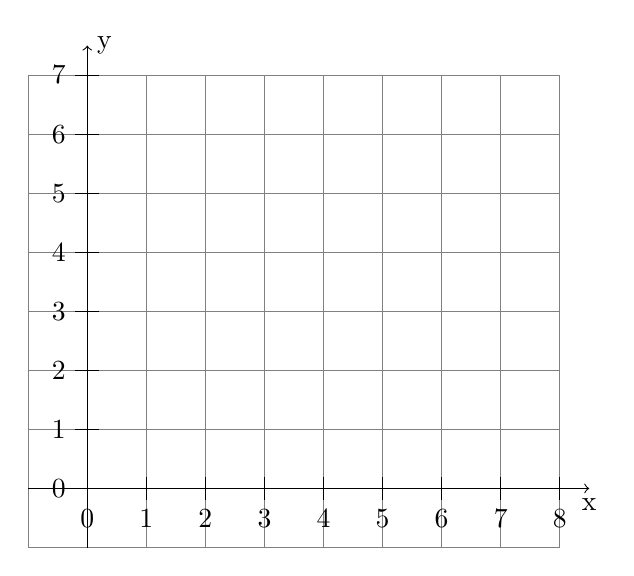
\begin{tikzpicture}[scale=0.75]
				\tikzset{
					grid major/.style = {very thin, gray},
					grid minor/.style = {very thin, lightgray}
				}
				\draw[grid major] (-1, -1) grid[step=1] (8, 7);
				\draw[->] (-1,0) -- (8.5,0) node[below] {x};
				\draw[->] (0,-1) -- (0,7.5) node[right] {y};
				\foreach \x in {0,1,...,8} \draw (\x,0.2) -- (\x,-0.2) node[below] {\x};
				\foreach \y in {0,1,...,7} \draw (0.2,\y) -- (-0.2,\y) node[left] {\y};

			\end{tikzpicture}
		\end{center}
	\end{multicols}
